\documentclass[a4paper]{article}
%\usepackage[singlespacing]{setspace}
\usepackage[onehalfspacing]{setspace}
%\usepackage[doublespacing]{setspace}
\usepackage{geometry} % Required for adjusting page dimensions and margins
\usepackage{amsmath,amsfonts,stmaryrd,amssymb,mathtools,dsfont} % Math packages
\usepackage{tabularx}
\usepackage{colortbl}
\usepackage{listings}
\usepackage{amsmath}
\usepackage{amssymb}
\usepackage{amsthm}
\usepackage{subcaption}
\usepackage{float}
\usepackage[table,xcdraw]{xcolor}
\usepackage{tikz-qtree}
\usepackage{changepage,titlesec,fancyhdr} % For styling Header and Titles
\pagestyle{fancy}

\usepackage{enumerate} % Custom item numbers for enumerations

\usepackage[ruled]{algorithm2e} % Algorithms

\usepackage[framemethod=tikz]{mdframed} % Allows defining custom boxed/framed environments

\usepackage{listings} % File listings, with syntax highlighting
\lstset{
	basicstyle=\ttfamily, % Typeset listings in monospace font
}

\usepackage[ddmmyyyy]{datetime}


\geometry{
	paper=a4paper, % Paper size, change to letterpaper for US letter size
	top=2.5cm, % Top margin
	bottom=3cm, % Bottom margin
	left=2.5cm, % Left margin
	right=2.5cm, % Right margin
	headheight=25pt, % Header height
	footskip=1.5cm, % Space from the bottom margin to the baseline of the footer
	headsep=1cm, % Space from the top margin to the baseline of the header
	%showframe, % Uncomment to show how the type block is set on the page
}
\lhead{ALGO-1\\Sommersemester 2024}
\chead{\bfseries{Übungsblatt 6}\\}
\rhead{7987847\\Jonas Werner}

\begin{document}
\section*{Aufgabe 7.1}
Gegeben sei der folgende (a, b)-Baum $T_{ab}$:

\begin{center}
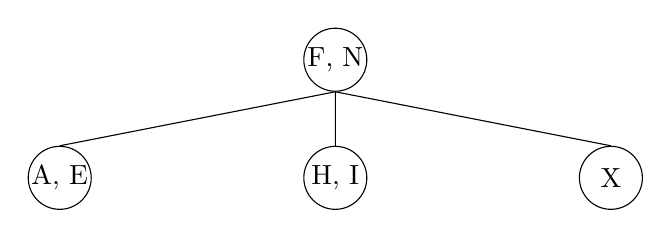
\begin{tikzpicture}[
  every node/.style = {draw, circle, minimum size=8mm, inner sep=0pt},
  level 1/.style={sibling distance=35mm},
  level 2/.style={sibling distance=20mm}
  ]
  \node {F, N}
    child {node {A, E}}
    child {node {H, I}}
    child {node {X}};
\end{tikzpicture}
\end{center}

Fügen Sie für die beiden folgenden Spezifikationen von Tab jeweils die Schlüssel C, Y, T, S und Q ein und entfernen Sie anschließend die Schlüssel N, A und S (jeweils in dieser Reihenfolge).

\begin{enumerate}
    \item[ a)] Tab ist ein (2, 3)-Baum.
    \item[ b)] Tab ist ein (2, 4)-Baum.
\end{enumerate}

Geben Sie jeweils die Zwischenschritte in graphischer Darstellung an und beschreiben Sie kurz, was - aus welchem Grund - geschieht.

\textbf{Hinweis:} Es kann für das Verständnis helfen, die Operationen noch einmal in kleinere Zwischenschritte aufzuspalten. Es genügt jedoch, eine Grafik für den Zustand nach jeder Operation anzugeben.

\subsection*{a)}

\begin{verbatim}
     (F,N)   insert(C)     (F,N)                (C,F,N)                  (F)    insert(Y)
    /  |  \     ->        /  |  \     ->        /  |  \     ->          /  \      ->
(A,E) (H,I) (X)      (A,C,E) (H,I) (X)      (A,E) (H,I) (X)         (C)     (N)
                                                                   /  \     /  \
                                                                (A)   (E) (H,I) (X)


         (F)                       (F)                        (F)           
        /  \       insert(T)      /  \                        /  \            insert(S)
     (C)     (N)      ->       (C)     (N)      ->        (C)      (N,X)        ->
   /  \     /  \             /  \     /  \               /  \     /   |  \  
(A)   (E) (H,I) (X,Y)     (A)   (E) (H,I) (T,X,Y)     (A)   (E) (H,I) (T) (Y)


         (F)                       (F)                        (F)           
        /  \       insert(Q)      /  \                        /  \             
     (C)      (N,X)    ->       (C)      (N,X)  ->        (C)      (N,S,X)        ->
   /  \     /   |  \         /  \     /   |  \           /  \     / |  |  \  
(A)   (E) (H,I)(S,T) (Y)  (A)   (E)(H,I)(Q,S,T) (Y)    (A)  (E)(H,I)(Q)(T) (Y)
\end{verbatim}
\break
\begin{verbatim}
         
         (F,S)                       (F,S)              
      /   |    \     remove(N)     /   |    \             
    (C)  (N)     (X)    ->      (C)  ( )     (X)      ->
   / \   /  \     /  \        / \   /  \     /  \ 
(A)  (E)(H,I)(Q) (T) (Y)  (A)  (E)(H,I)(Q)  (T) (Y)


         (F,S)                       (F,S)              
      /   |    \                   /   |    \        remove(A)
    (C)  (Q)     (X)    ->      (C)   (I)    (X)      ->
   / \    |     /  \            / \   / \    / \ 
(A)  (E)(H,I)  (T) (Y)       (A) (E) (H)(Q) (T) (Y)



         (F,S)                       (F,S)              
      /   |    \                   /   |    \             
    (C)  (Q)     (X)    ->      ( )   (I)    (X)      ->
   / \    |     /  \            /     / \    / \ 
( )  (E)(H,I)  (T) (Y)       (C,E)  (H) (Q) (T) (Y)


         (S)                         ( )              
      /       \    remove(s)      /        \             
    (F,I)      (X)    ->        (F,I)      (X)     ->
   /  |  \    /  \             /  |  \    /  \  
(C,E)(H) (Q) (T) (Y)        (C,E)(H) (Q) (T) (Y)


         (T)                         (T)              
      /       \                   /        \             
    (F,I)      (X)    ->        (F,I)      ( )     ->
   /  |  \    /  \             /  |  \      |  
(C,E)(H) (Q) ( ) (Y)        (C,E)(H) (Q)  (X,Y)


         (I)              
      /      \             
    (F)      (T)     
   /  \      /  \ 
(C,E) (H)  (Q) (X,Y)

\end{verbatim}


\subsection*{b)}

\begin{verbatim}
     (F,N)  insert(C)      (F,N)  insert(Y)       (F,N)  insert(T)       (F,N)  insert(S)
    /  |  \     ->        /  |  \     ->       /   |   \    ->         /   |   \      ->
(A,E) (H,I) (X)      (A,C,E) (H,I) (X)    (A,C,E) (H,I) (X,Y)    (A,C,E) (H,I) (T,X,Y)


         (F,N)                      (F,N,T)   insert(Q)      (F,N,T)   remove(N)
      /   |    \     ->            /  |   | \     ->       /  |   | \   ->
(A,C,E) (H,I) (S,T,X,Y)      (A,C,E)(H,I)(S)(X,Y)    (A,C,E)(H,I)(Q,S)(X,Y)


         (F,T)                        (F,Q,T)      remove(S)   (F,Q,T)
      /   |   |   \    ->            /  |   | \     ->       /  |   | \
(A,C,E) (H,I)(Q,S)(X,Y)         (A,C,E)(H,I)(S)(X,Y)  (A,C,E)(H,I)  ( )(X,Y)


         (F,Q,T)                        (F,I,T)
      /   |   |   \    ->            /  |  |  \ 
(A,C,E) (H,I)( )(X,Y)           (A,C,E)(H)(Q)(X,Y)

\end{verbatim}

\section*{Aufgabe 7.2 Nahezu sortiert (18 Punkte)}

Sei A ein Array mit \( n > 0 \) natürlichen Zahlen, wobei keine Zahl mehr als einmal vorkommt. Die Einträge in A seien bezüglich eines Parameters \( k \leq n \) "nahezu" sortiert, d.h., jeder Eintrag ist höchstens um \( k \) Positionen von seiner eigentlich korrekten Position in der Sortierung entfernt.

Entwerfen Sie einen Algorithmus, der die Einträge im Array A in die korrekte Sortierung überführt. Die Laufzeit sollte \( O(n \log k) \) nicht überschreiten. Beschreiben Sie wie immer zuerst die Idee Ihres Algorithmus und geben Sie ihn dann in Pseudocode an. Zeigen Sie, dass der Algorithmus korrekt arbeitet und die genannte Laufzeitschranke einhält.





\end{document}